%%%%%%%%%%%%%%%%%%%%%%%%%%%%%%%%%%%%%%%%%%%%%%%%%%%%%%%%%%%%%%%%%%%%%%%%%%%%%%%%%%%%%%%%%%
\section{Discussion} \label{sec:discussion} 

%%%%%%%%%%%%%%%%%%%%%%%%%%%%%%%%%%%%%%%%%%%%%
\subsection{Feature selection}

% sklearn random forest  

\begin{table}[H]
    \centering
    \caption{Ranking of feature importance from best to worst with respect to
    impurity decrease for three different reconstruction methods on the full
    dataset obtained with sci-kit learn.}  
    \label{tab:feature_importance}  

    \begin{tabular}{|c|c|c|c|}
        \hline
        Rank & Feature index & Feature name & Impurity decrease \\     
        \hline
        0       & 2           & histogram min  & 0.102915  \\
        1      & 12            & glcm entropy  & 0.088981  \\
        2      & 11           & glcm contrast  & 0.083777  \\
        3       & 4           & histogram std  & 0.081181  \\
        4      & 13        & glcm homogeneity  & 0.080463  \\
        5       & 5      & shape area\_density  & 0.073690  \\
        6       & 3          & histogram peak  & 0.069483  \\
        7       & 0           & histogram max  & 0.064857  \\
        8      & 14      & glcm joint\_maximum  & 0.061548  \\
        9       & 9    & shape volume\_density  & 0.055089  \\
        10      & 8            & shape volume  & 0.051088  \\
        11      & 7           & shape surface  & 0.048897  \\
        12     & 10            & glcm cluster  & 0.048494  \\
        13      & 1          & histogram mean  & 0.047758  \\
        14      & 6  & shape convex\_hull\_area  & 0.041778  \\
        \hline
         
    \end{tabular} 
\end{table}


% Identify features with poor class separation

% Identify highly correlated features  
% * plot correlation matrix  

\begin{figure}[H]
    \centering
    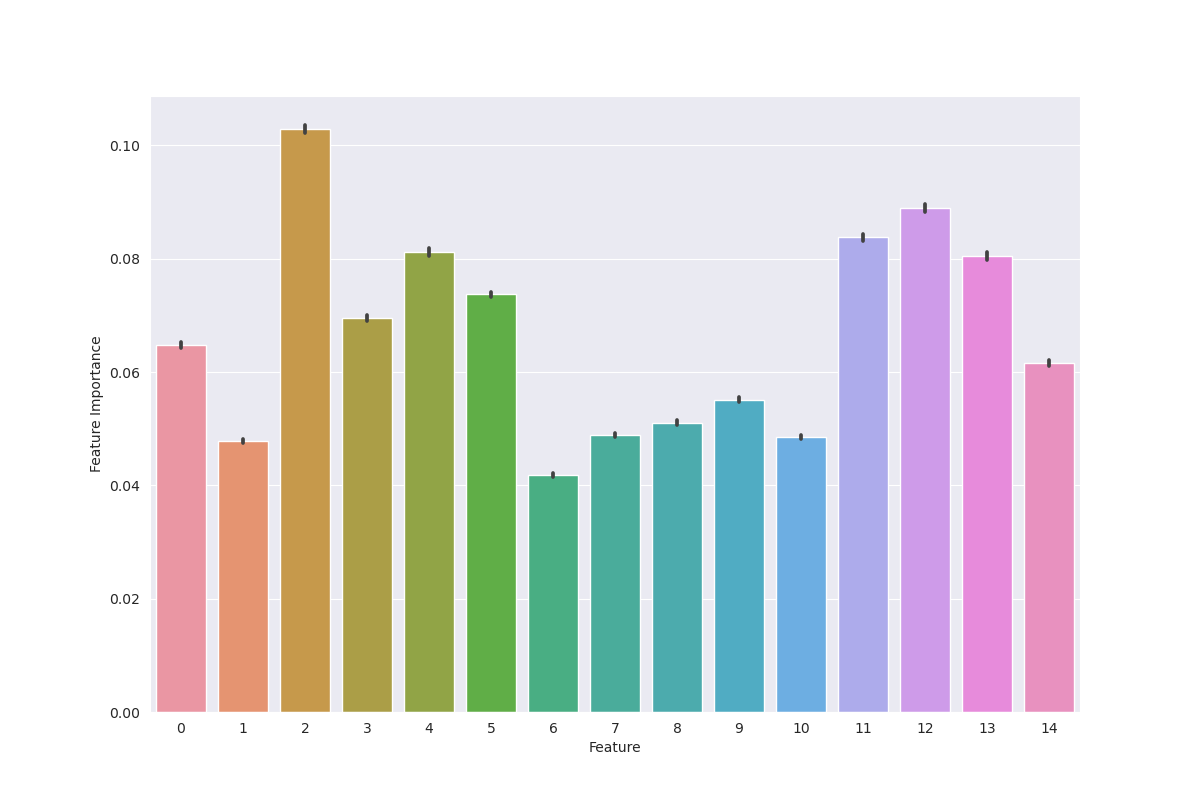
\includegraphics[width=0.8\textwidth]{Figures/feature_importance_sklearn_3s.png}
    \caption{Mean of the feautre\_importacnes\_ (purity decrease) for each decision tree. The
    error bar shows the 95\% confidence interval. The x-axis represent feature
    number as defined in table \ref{tab:feature_names}.  }  
    \label{fig:feature_importance} 
\end{figure}

% \begin{figure}[H]
%     \centering
%     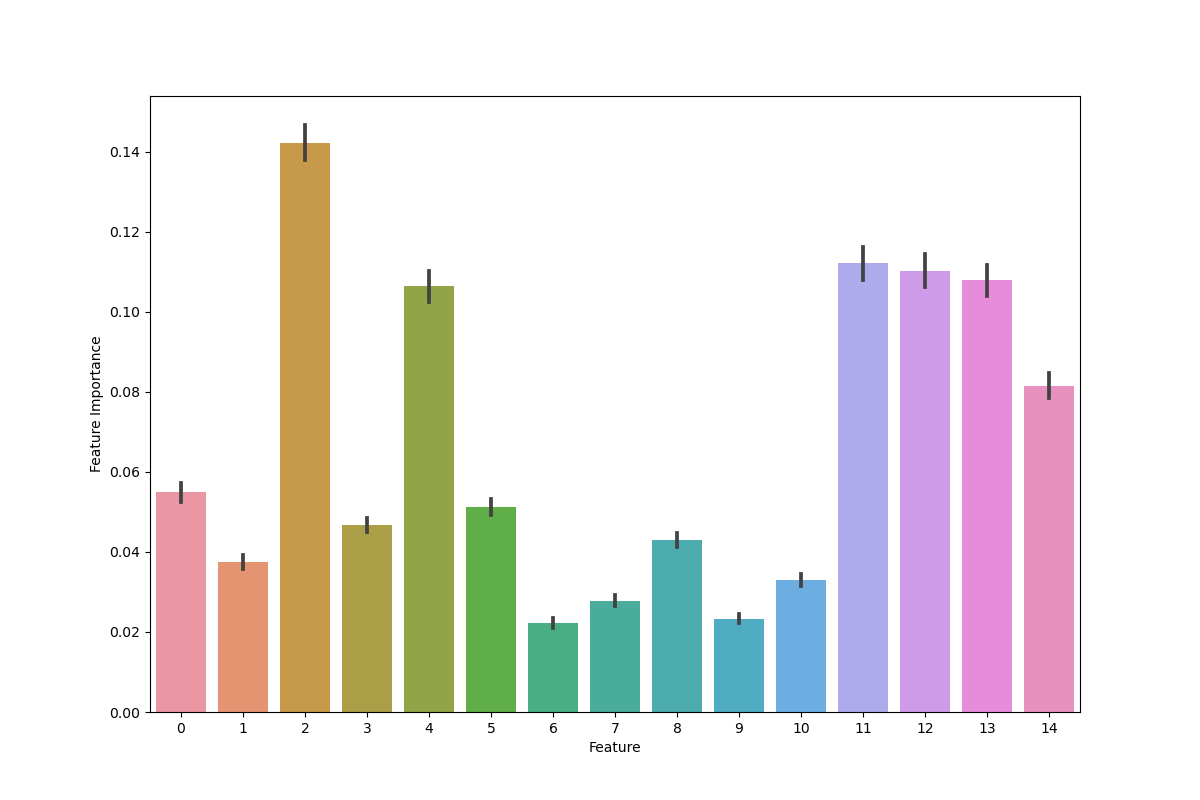
\includegraphics[width=0.8\textwidth]{Figures/feature_importance.png}
%     \caption{Mean of the feautre\_importacnes\_ (purity decrease) for each decision tree. The
%     error bar shows the 95\% confidence interval. The x-axis represent feature
%     number as defined in table XXX: ref table.  }  
%     \label{fig:feature_importance} 
% \end{figure}

Figure \ref{fig:feature_importance} shows the histogram the feature importance
on the y axis and feature index on the x axis. These results was obtained with
with sci-kit learn's implementation of the random forest. The 95 \% confidence
interval is shown on the top of each bar. The histogram min is best able to
discriminate between the tree different reconstruction methods, with a impurity
decrease of 0.1029\&. The numerical feature importance (Impurity decrease)
values for all the features is listed in table \ref{tab:feature_importance}.
The glcm entropy features gives the second best impurity decrease with a value
of 0.0890. Our next 3 best features are glcm contrast, histogram std and glcm
homogeneity which performs similarity with an impurity descrese in the rande
0.0805-0.0838. 

In figure \ref{fig:correlation} the correlation between all the features is
plotted. The color bar has a range from -1 (black) to 1 (white), where a score
of 1 indicates perfect correlation. The histogram min features is not strongly
correlated with any other features, thus we expect this features give a good
accuracy on the test data with the SVM model. Our next best features glcm
entorpy is highly correlated with histogram std. Thus, only one of the features
should be used when training a classification model. Utilizing both features
will produce high variance due to redundant information. When training our SVM
we therefore expect the combinations of these two features to produce worse
accuracy on the test data compared with any other combination of the top 5
features. Glcm contrast has the highest correlation with histogram std, but not
to the same extent as the two previous discussed features. GLCM homogeneity has
the highest correlation with glcm joint\_maximum. However, the GLCM maximum
features performance significantly worse with a difference impurity decrease of
0.0189. In our training of the SVM we expect that a combination of hisogram
min, glcm entropy. The 4 combinations of features we expect to
produce the best predication on the test data is listed in table
\ref{tab:expectation}. Also, every combination of two features in each row is
expected perform well with SVM. 

\begin{table}
    \centering
    \caption{Each row corresponds to a set of feature combinations that is
        expected to give good accuracy with SVM. Combinations of two of the features
    in each row shoud also give good accuracy with SVM. The columns is sorted
with respect to impurity decrease, where the left most column has the highest
impurity decrease}  
    \label{tab:expectation} 
    \begin{tabular}{|c|c|c|}
        \hline
        feature 1 & feature 2 & feature 3 \\
        \hline
        histogram min & gclm entropy & glcm homogeneity \\ 
        histogram min & gclm entropy & histogram std  \\ 
        histogram min & gclm contrast & glcm homogeneity \\ 
        histogram min & gclm contrast & histogram std  \\ 
        \hline
    \end{tabular} 
\end{table}

\begin{figure}[H]
    \centering
    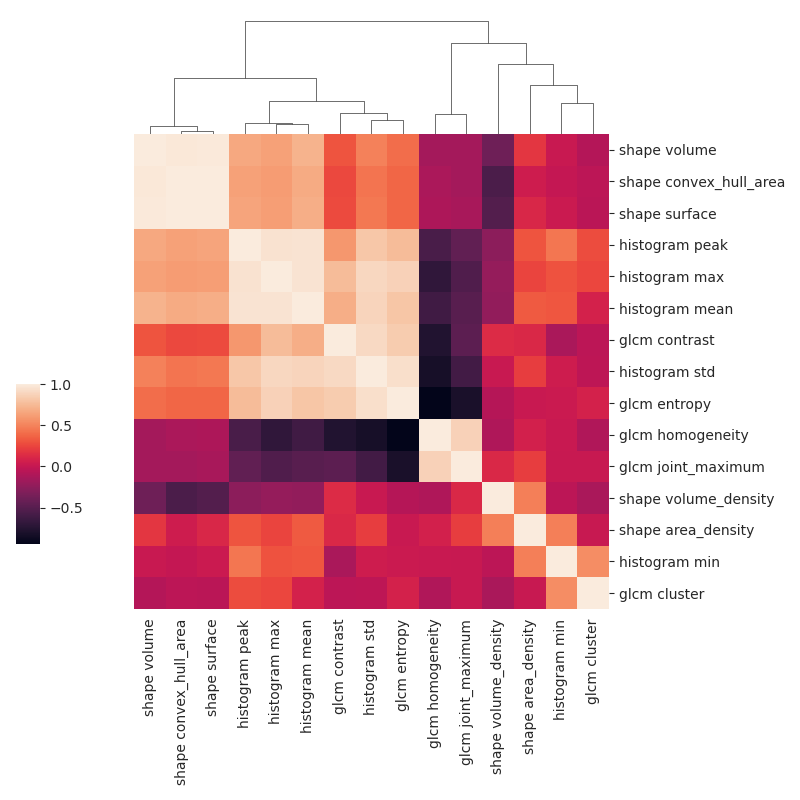
\includegraphics[width=1\textwidth]{Figures/feature_correlation.png}
    \caption{Pearson Correlation between each feature calculated on the full
    dataset. }  
    \label{fig:correlation} 
\end{figure}








%%%%%%%%%%%%%%%%%%%%%%%%%%%%%%%%%%%%%%%%%%%%
\subsection{SVM}

\subsubsection{Classification of series PT-PET-EARLAC vs PT-PET-WB-Q-CLEAR}
\label{sec:SVM0}
This sub sub section provides results from the SVM classifying series 1 named \verb|PT_PET_EARLAC|
versus series 2 named \verb|PT_PET_WB_Q_CLEAR|. 

\begin{figure}[H]
\centering
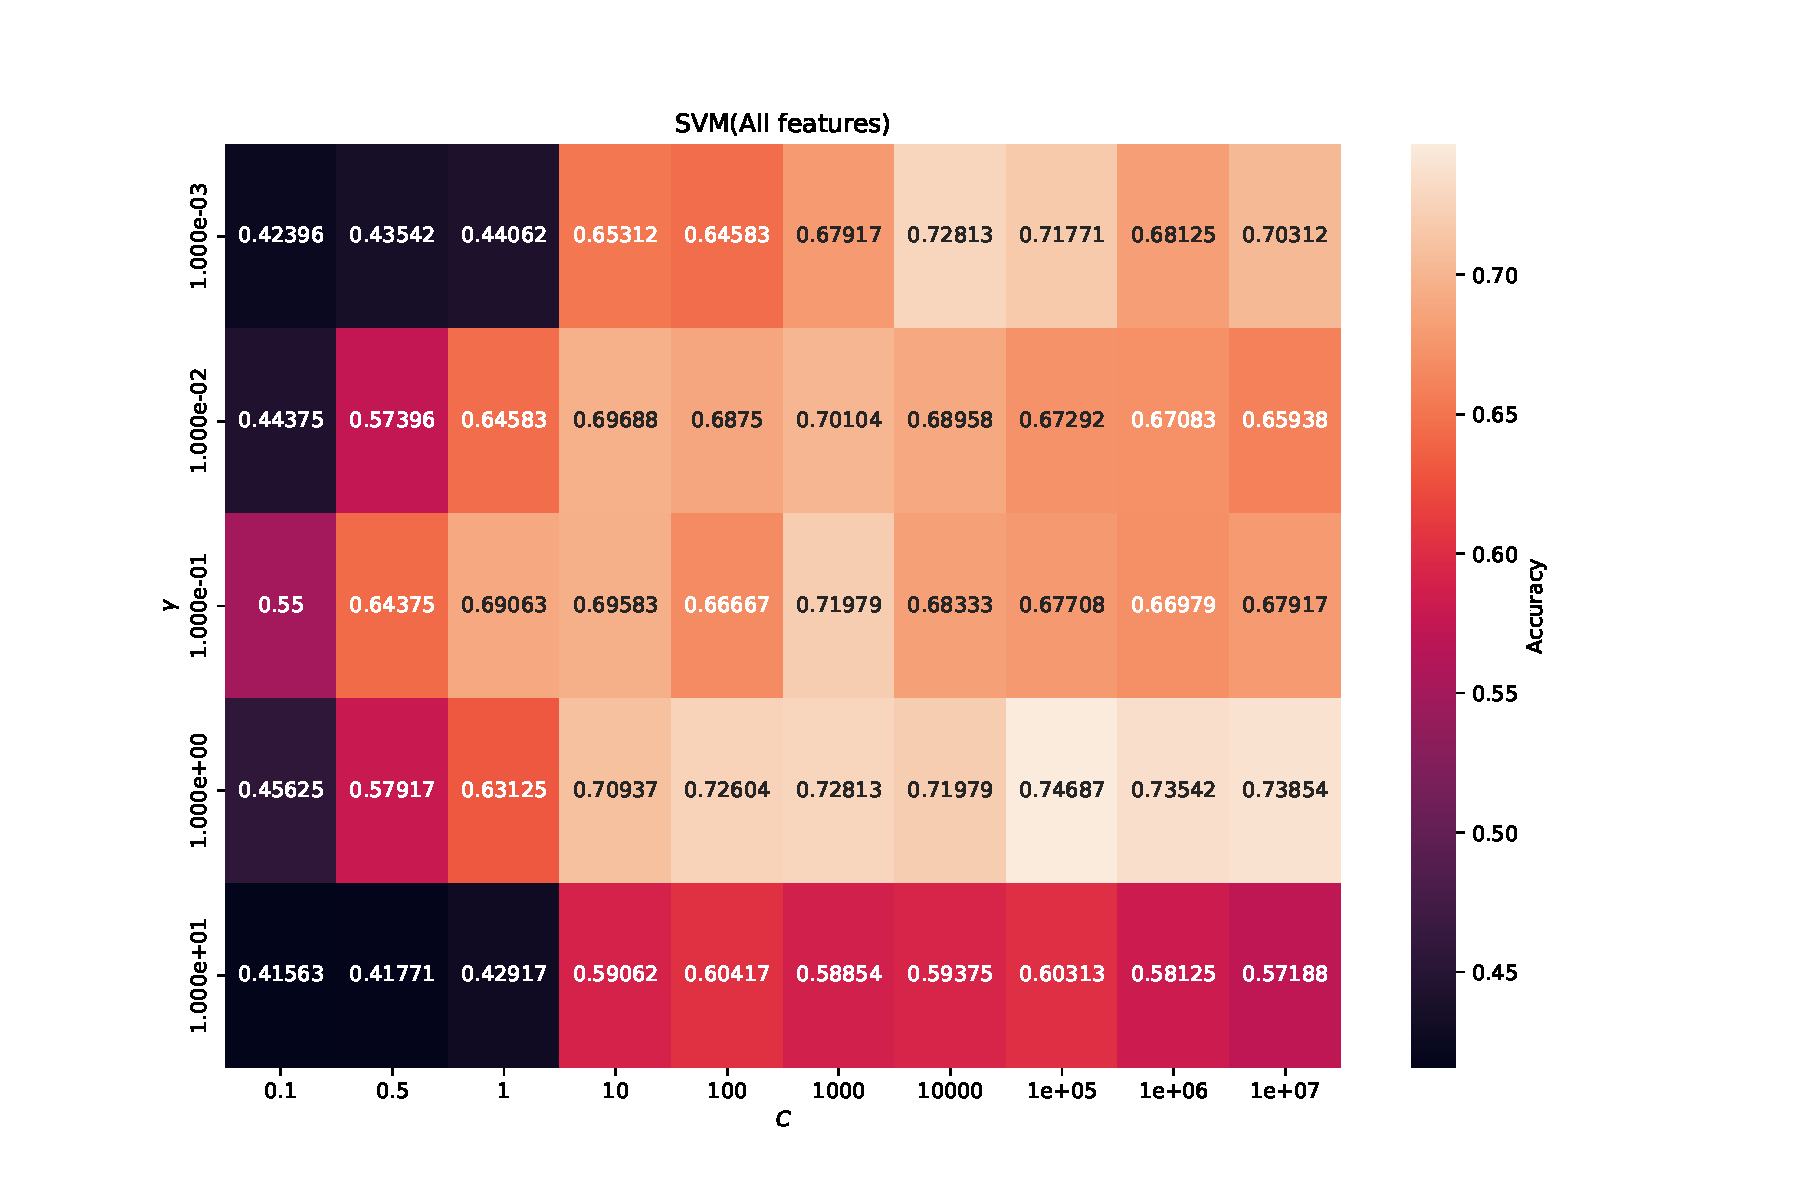
\includegraphics[width=1\textwidth]{Figures/accuracy(C,gamma)0}
\caption{Heatmap of the accuracy obtained with different slack constants $C$ and 
GRBF kernel factors $\gamma $ in the SVM model training with all the features. The SVM accuracies are the average of $30$ cross-validation 
cycles training and predicting test data of relative size $0.25$.
The predictions are wither the data belongs to series 1 or 2.}
\label{fig:Figures-accuracy-C-gamma-0}
\end{figure}
\autoref{fig:Figures-accuracy-C-gamma-0} shows the accuracy of the SVM model's 
test data predictions for different slack constants $C$ and GRBF kernel factors $\gamma $. 
We observe the best accuracy $0.747$ for $C=10^5$ and $\gamma =1$. Lower slack constant 
allows for more misclassification while lower $\gamma $ results in a wider 
GRBF kernel which means that the influence of each data point on the hyperplane 
position will decrease. Both leads towards under fitting on the under-over fit spectrum.
Our optimal values for $C$ and $\gamma $ are quite large suggesting the need for 
a complex hyperplane to classify our data. 

We will utilize these optimal value in our analysis of predictions based on two and three 
features. They should be tuned for every feature combination, but this would required 
way to much computation to handle for our computer. The optimal parameter values 
obtained using all the features will be good general parameters for the following 
feature combination analysis. 

\begin{figure}[H]
\centering
\makebox[\textwidth][c]{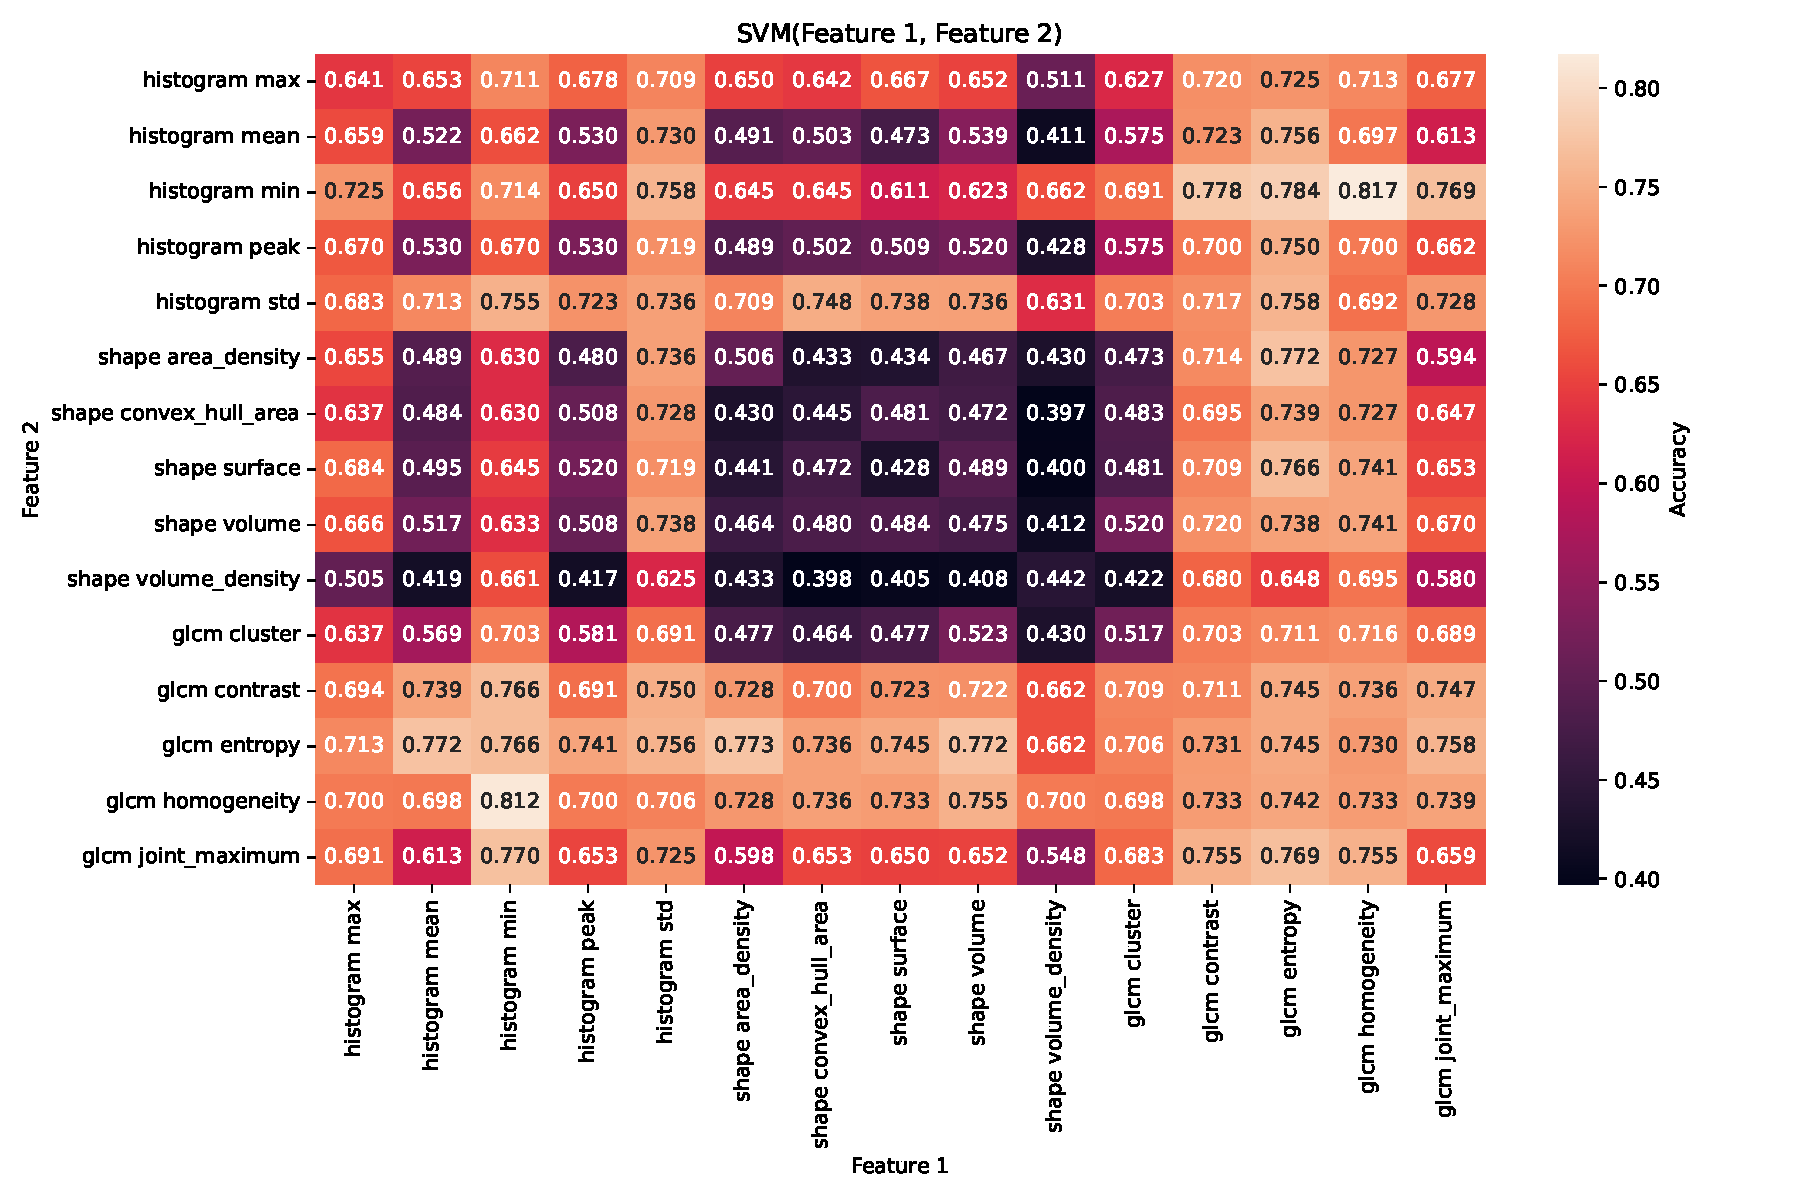
\includegraphics[width=1.2\textwidth]{Figures/feature_pairs0}}
\caption{Heatmap of the accuracy obtained by the SVM model training on different feature pairs. The SVM accuracies are the average 
of $20$ cross-validation cycles training and predicting test data of relative size $0.25$.
The slack constant and GRBF kernel factor are set to $C=10^5$ and $\gamma=1 $ respectively.
 The predictions are wither the data belongs to series 1 or 2.}
\label{fig:Figures-feature_pairs0}
\end{figure}

\autoref{fig:Figures-feature_pairs0} shows a heatmap of the accuracy obtained with different 
feature pairs utilized by the SVM model for training and predicting. The diagonal from upper left 
to lower right of the heatmap shows pairs of same features which is equivalent to classification 
based on that single feature. We observe the best score for a single feature with \verb|glcm entropy|
with accuracy $0.745$.

The accuracy of each feature pairs have been derived twice, one on either side of the equal feature diagonal, which is nice as 
this gives some conformation. We observe both scores of the feature pair \verb|histogram min| and \verb|glcm homogeneity| 
to be the best with accuracy $0.812$ and $0.817$. This feature pair is one of the combinations 
expected to give good results in \autoref{tab:expectation}. The table also shows an expected 
good result with the feature pair \verb|glcm entropy| and \verb|glcm homogeneity|, although 
our SVM analysis shows worse accuracy when including \verb|glcm homogeneity| compared to \verb|glcm entropy| 
alone. Assuming these features have low correlation as shown in \autoref{fig:correlation}, one would expect 
an increase in accuracy as both shows good accuracy on their own. Therefore the poor accuracy 
might be a result of bad parameters ($C$ and $\gamma $) for this combination of feature. The rest of the 
feature pair combinations in the rows of \autoref{tab:expectation} seem to improve the accuracy. 

\begin{figure}[H]
\centering
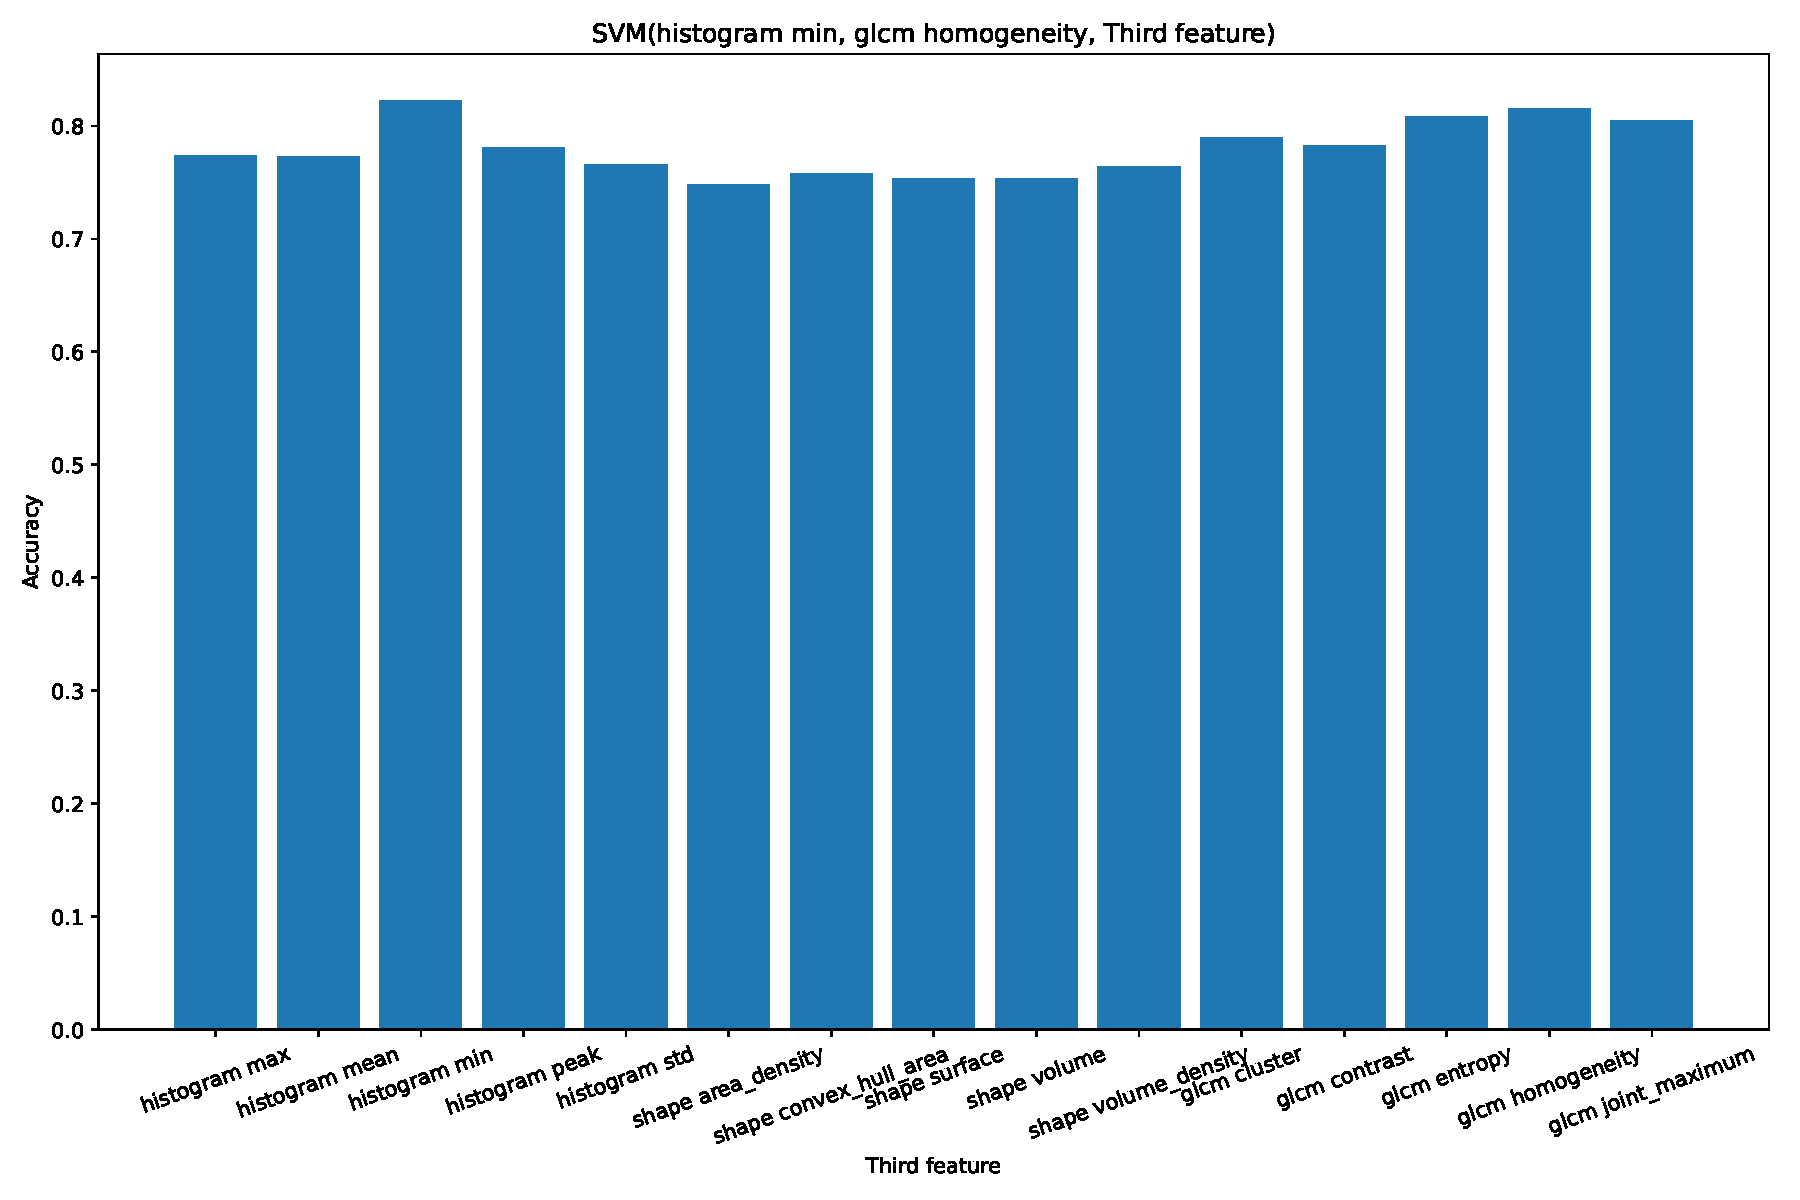
\includegraphics[width=1\textwidth]{Figures/third_feature0}
\caption{Bar plot of the accuracy obtained adding a third feature in the data used 
by the SVM model. The accuracies are the average 
of $50$ cross-validation cycles training and predicting test data of relative size $0.25$.
The slack constant and GRBF kernel factor are set to $C=10^5$ and $\gamma=1 $ respectively.
 The predictions are wither the data belongs to series 1 or 2.}
\label{fig:Figures-third_feature0}
\end{figure}

\autoref{fig:Figures-third_feature0} shows the accuracy gotten when adding a third feature to the best scoring feature pair 
\verb|histogram min| and \verb|glcm homogeneity| from \autoref{fig:Figures-feature_pairs0}. We observe best scores for 
third feature \verb|histogram min| and \verb|glcm homogeneity| which corresponds to no third feature. Thus, the addition of 
a third feature results in worse accuracy. The optimal feature pair in got better accuracy than 
what was obtained using all the features in \autoref{fig:Figures-accuracy-C-gamma-0} for which the parameters was tuned.
This suggest that there will be a point where adding more feature will decrease the prediction power of our model. 
Our results suggesting this point is for our two features should again be confirmed tuning the parameters $C$ and $\gamma $ 
for each third feature.  

\subsubsection{Classification of series PT-PET-EARL2 vs PT-PET-WB-Q-Clear}
\label{sec:SVM1}

This sub sub section provides results from the SVM classifying series 0 named \verb|PT_PET_EARL2|
versus series 2 named \verb|PT_PET_WB_Q_CLEAR|. 

\begin{figure}[H]
\centering
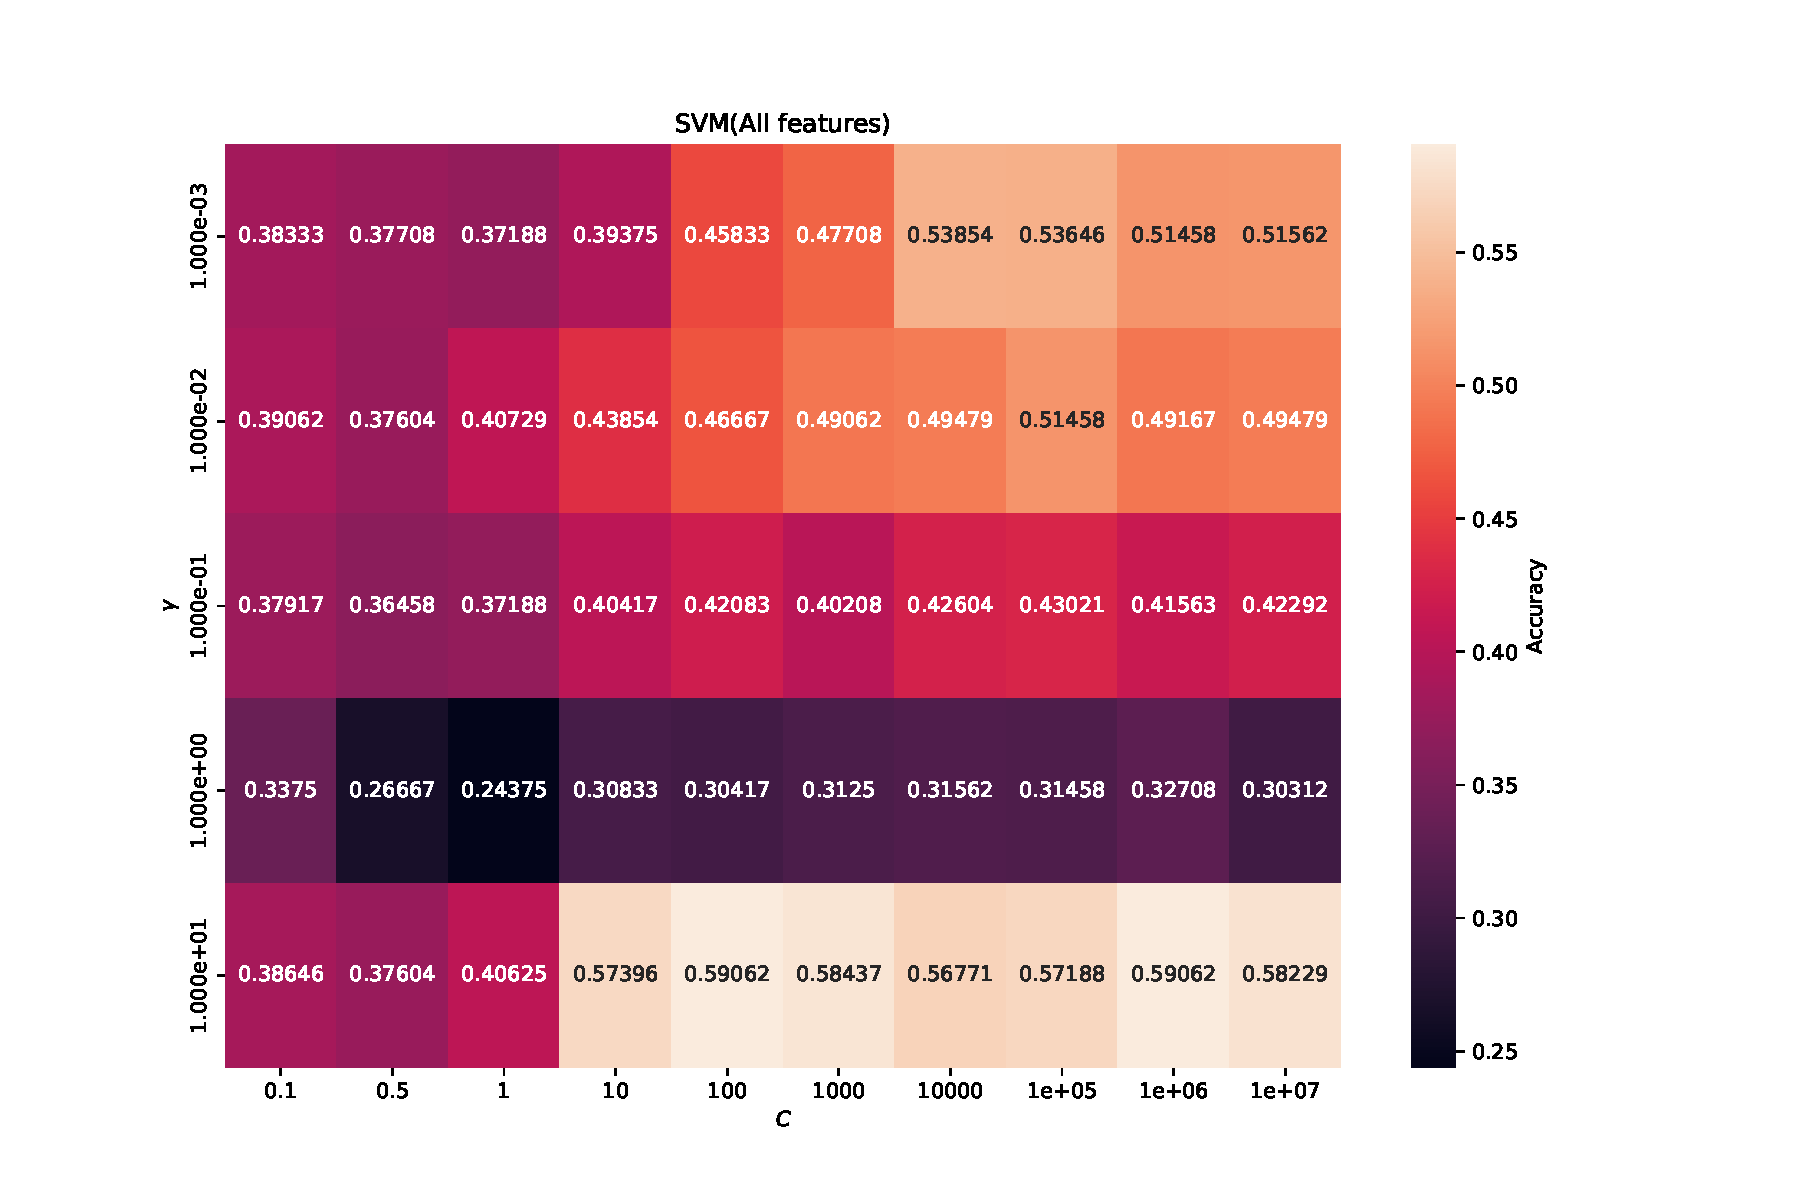
\includegraphics[width=1\textwidth]{Figures/accuracy(C,gamma)1}
\caption{Heatmap of the accuracy obtained with different slack constants $C$ and 
GRBF kernel factors $\gamma $ in the SVM model training with all the features. The SVM accuracies are the average of $30$ cross-validation 
cycles training and predicting test data of relative size $0.25$.
 The predictions are wither the data belongs to series 0 or 2.}

\label{fig:Figures-accuracy-C-gamma-1}
\end{figure}

\begin{figure}[H]
\centering
\makebox[\textwidth][c]{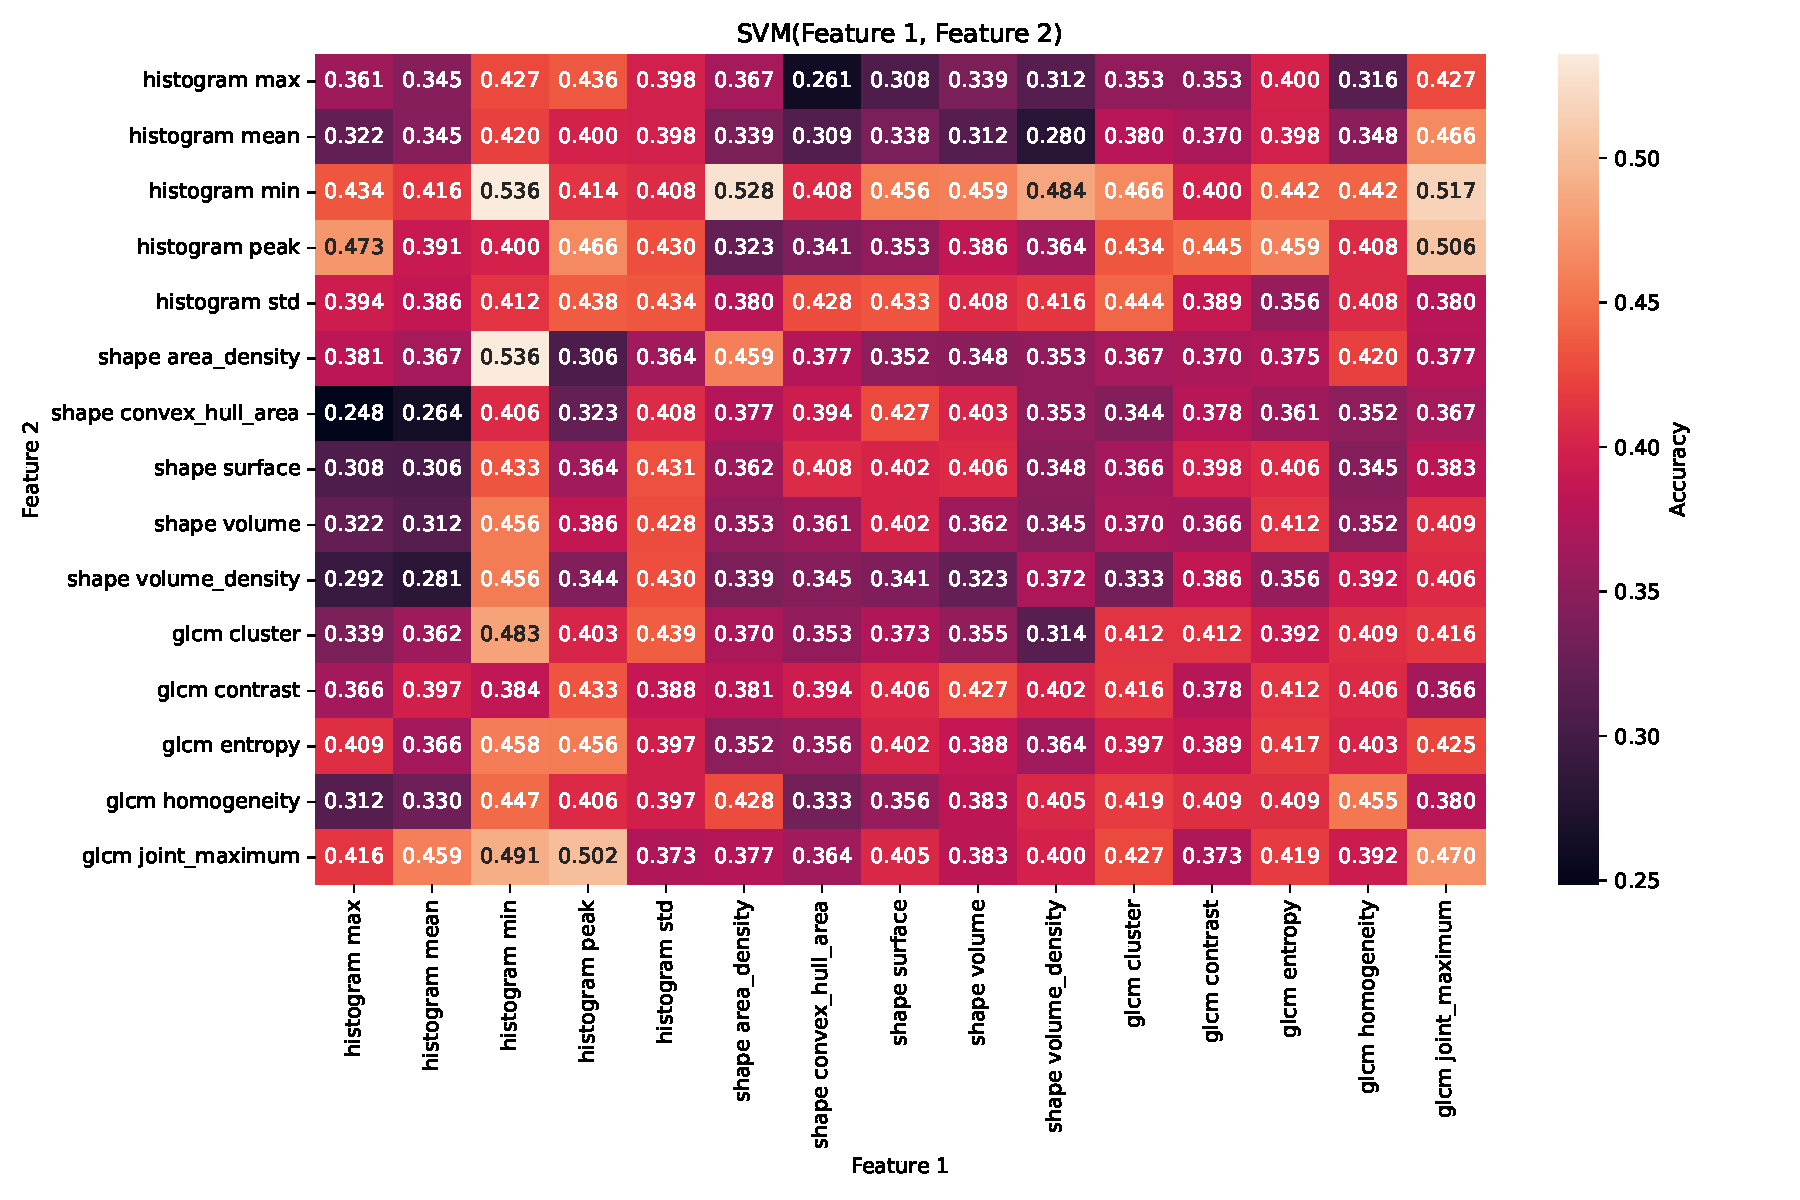
\includegraphics[width=1.2\textwidth]{Figures/feature_pairs1}}
\caption{Heatmap of the accuracy obtained by the SVM model training on different feature pairs. The SVM accuracies are the average 
of $20$ cross-validation cycles training and predicting test data of relative size $0.25$.
The slack constant and GRBF kernel factor are set to $C=100$ and $\gamma=10 $ respectively. 
 The predictions are wither the data belongs to series 0 or 2.}
\label{fig:Figures-feature_pairs1}
\end{figure}

\begin{figure}[H]
\centering
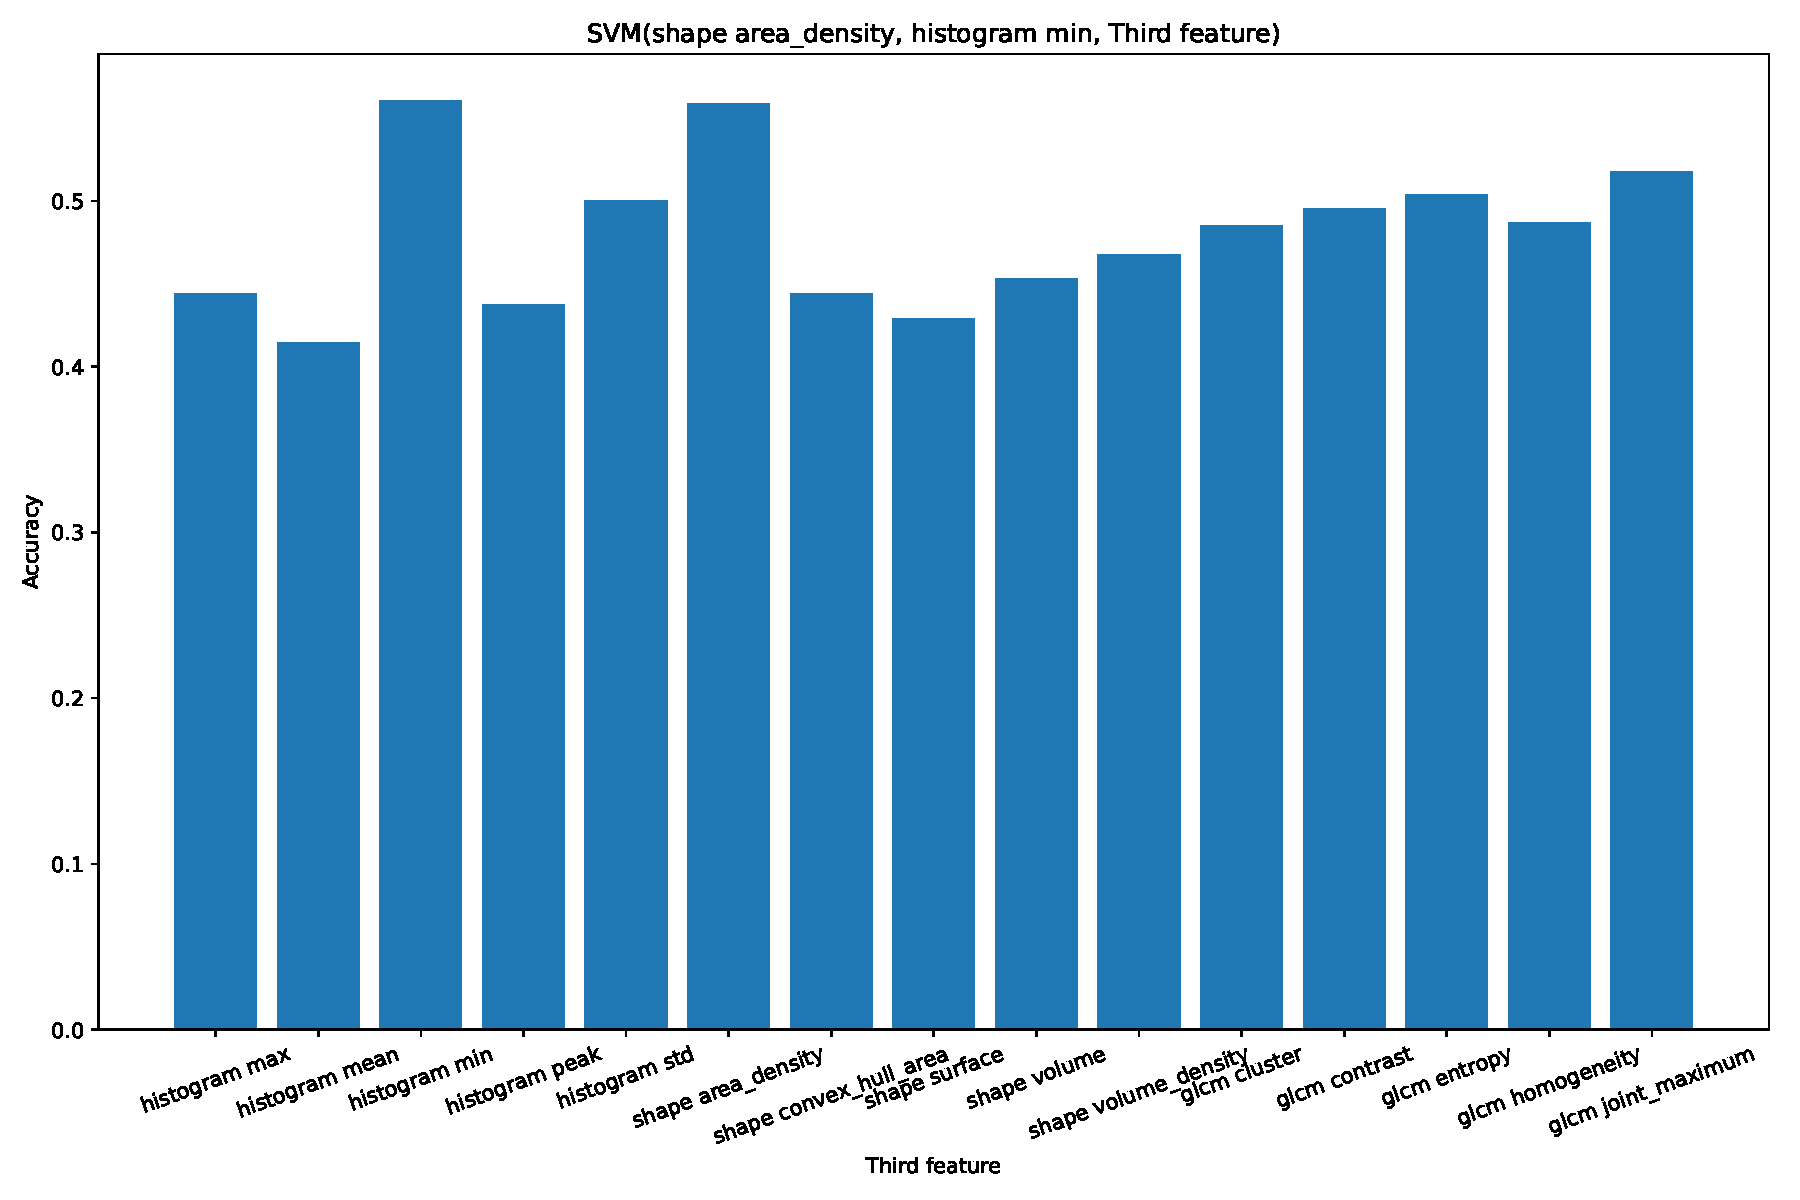
\includegraphics[width=1\textwidth]{Figures/third_feature1}
\caption{Bar plot of the accuracy obtained adding a third feature in the data used 
by the SVM model. The accuracies are the average 
of $50$ cross-validation cycles training and predicting test data of relative size $0.25$.
The slack constant and GRBF kernel factor are set to $C=100$ and $\gamma=10 $ respectively. 
 The predictions are wither the data belongs to series 0 or 2.}
\label{fig:Figures-third_feature1}
\end{figure}

\autoref{fig:Figures-accuracy-C-gamma-1}-\autoref{fig:Figures-third_feature1} shows the same figures as in \autoref{sec:SVM0}, but now 
classifying series 0 versus series 1 instead of series 1 versus series 2.

\autoref{fig:Figures-accuracy-C-gamma-1} shows the best accuracy of $0.591$  for $C=100$ and $\gamma =10$.
Utilizing these parameters, \autoref{fig:Figures-feature_pairs1} shows that the best feature pair accuracy $0.536$ was gotten with the feature pair 
\verb|shape area_density| and \verb|histogram min| where the latter also gave best accuracy $0.536$ when only using one feature.
From \autoref{fig:Figures-third_feature1}, we observe the addition of a third feature results in worse accuracy. 
The accuracies from single and pair features in \autoref{fig:Figures-feature_pairs1} are worse than what was obtain 
with all features. 

These results suggests the need for tuning the parameters for each feature combination utilized. 
This is especially visible in \autoref{fig:Figures-feature_pairs1} as the worst accuracies are further from accuracy $0.5$ than 
the best accuracies. This is because a useless model would have expected accuracy $0.5$ as each classification contains 50\% of the data. 
The trend is also visible in \autoref{fig:Figures-accuracy-C-gamma-1} such that the parameters when using all features 
should be more fine tuned. We may actually use the feature combinations giving the worst accuracies as the most predictive combinations 
by just classifying opposite to the model classification. Taking this into account we find 
the feature pair \verb|shape convex_hull_area| and \verb|histogram max| as well as the single feature 
\verb|histogram mean| to be most predictive with accuracies $1-0.248=0.752$ and $1-0.345=0.655$ respectively.  
Also, the best most predictive parameters in \autoref{fig:Figures-accuracy-C-gamma-1} are actually $C=1$ and $\gamma =1$
leading to a accuracy of $1-0.244=0.756$.  


\subsubsection{Classification of series PT-PET-EARL2 vs PT-PET-EARLAC}
\label{sec:SVM2}
This sub sub section provides results from the SVM classifying series 0 named \verb|PT_PET_EARL2|
versus series 1 named \verb|PT_PET_EARLAC| . 


\begin{figure}[H]
\centering
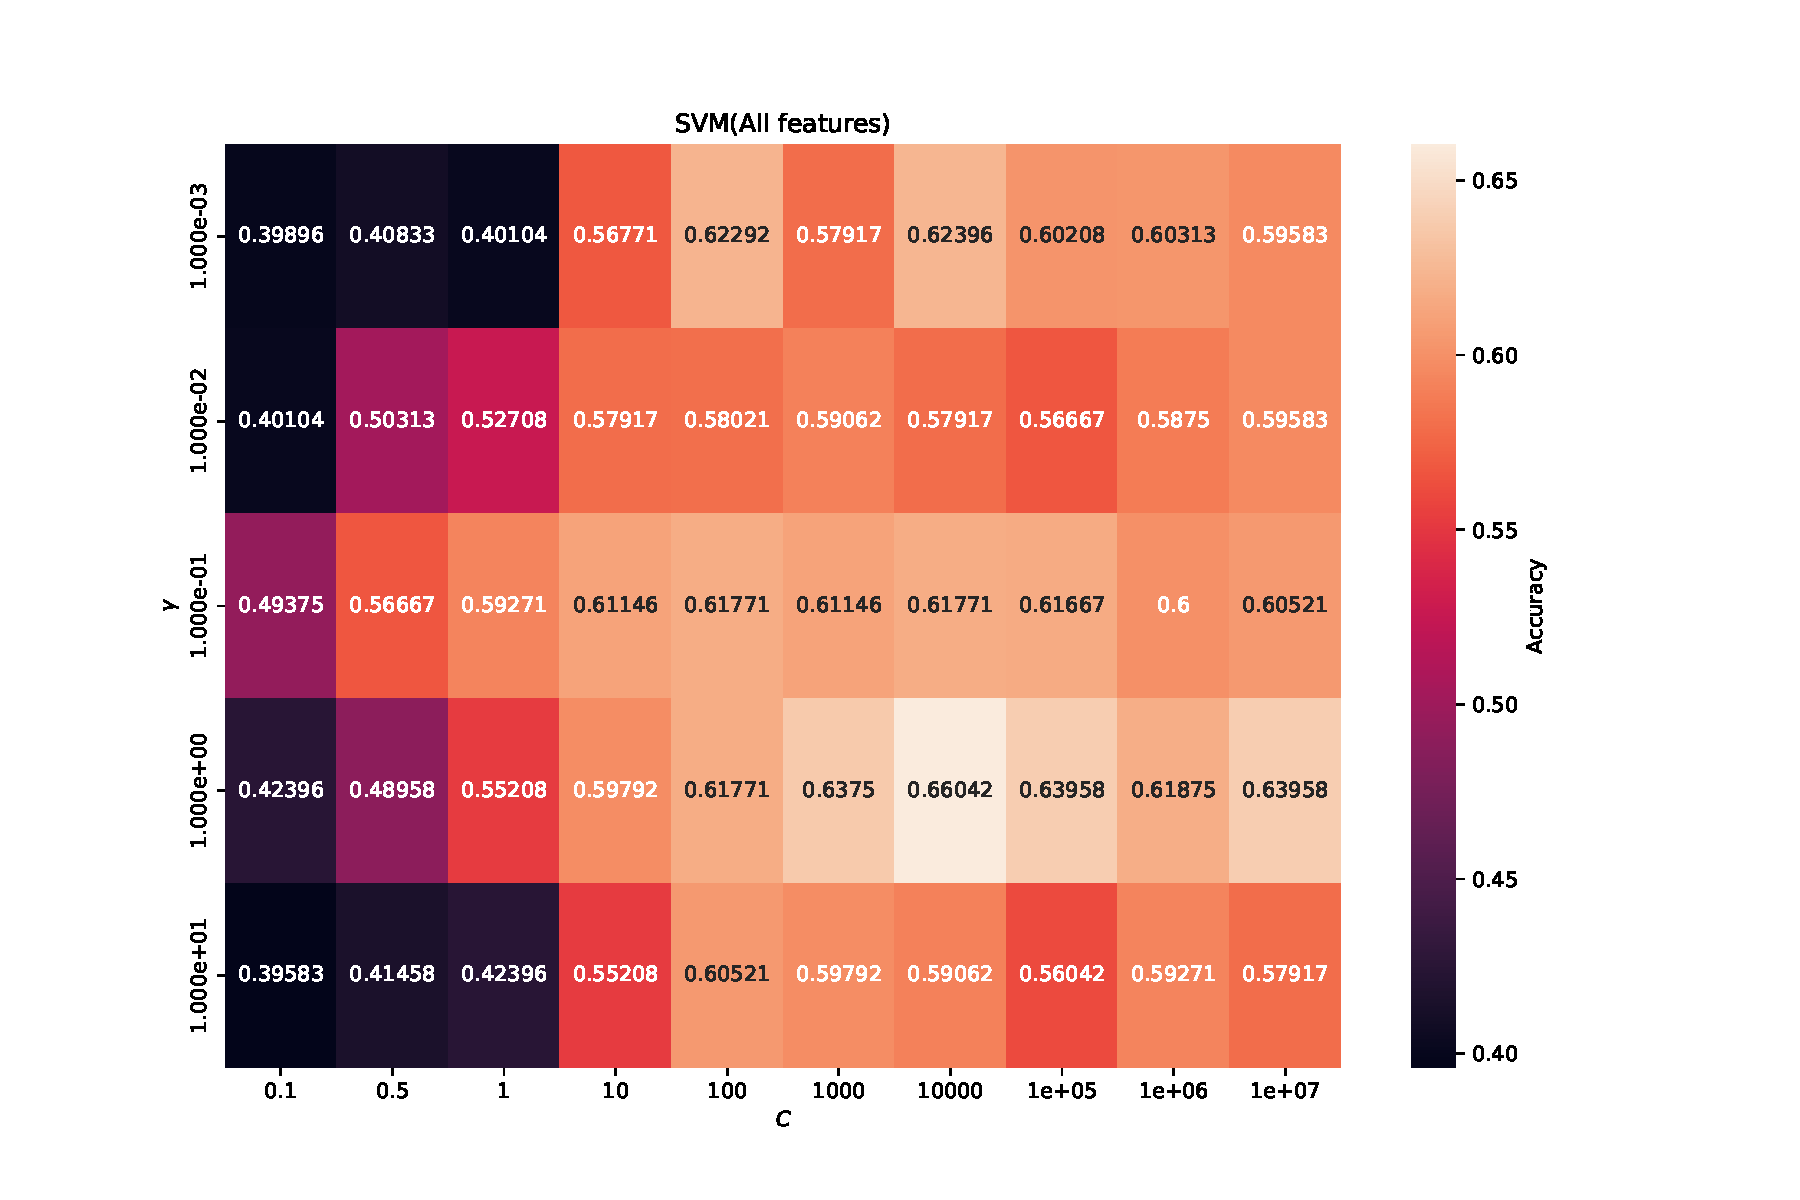
\includegraphics[width=1\textwidth]{Figures/accuracy(C,gamma)4}
\caption{Heatmap of the accuracy obtained with different slack constants $C$ and 
GRBF kernel factors $\gamma $ in the SVM model training with all the features. The SVM accuracies are the average of $30$ cross-validation 
cycles training and predicting test data of relative size $0.25$.
 The predictions are whether the data belongs to series 0 or 1.}
\label{fig:Figures-accuracy-C-gamma-4}
\end{figure}

\begin{figure}[H]
\centering
\makebox[\textwidth][c]{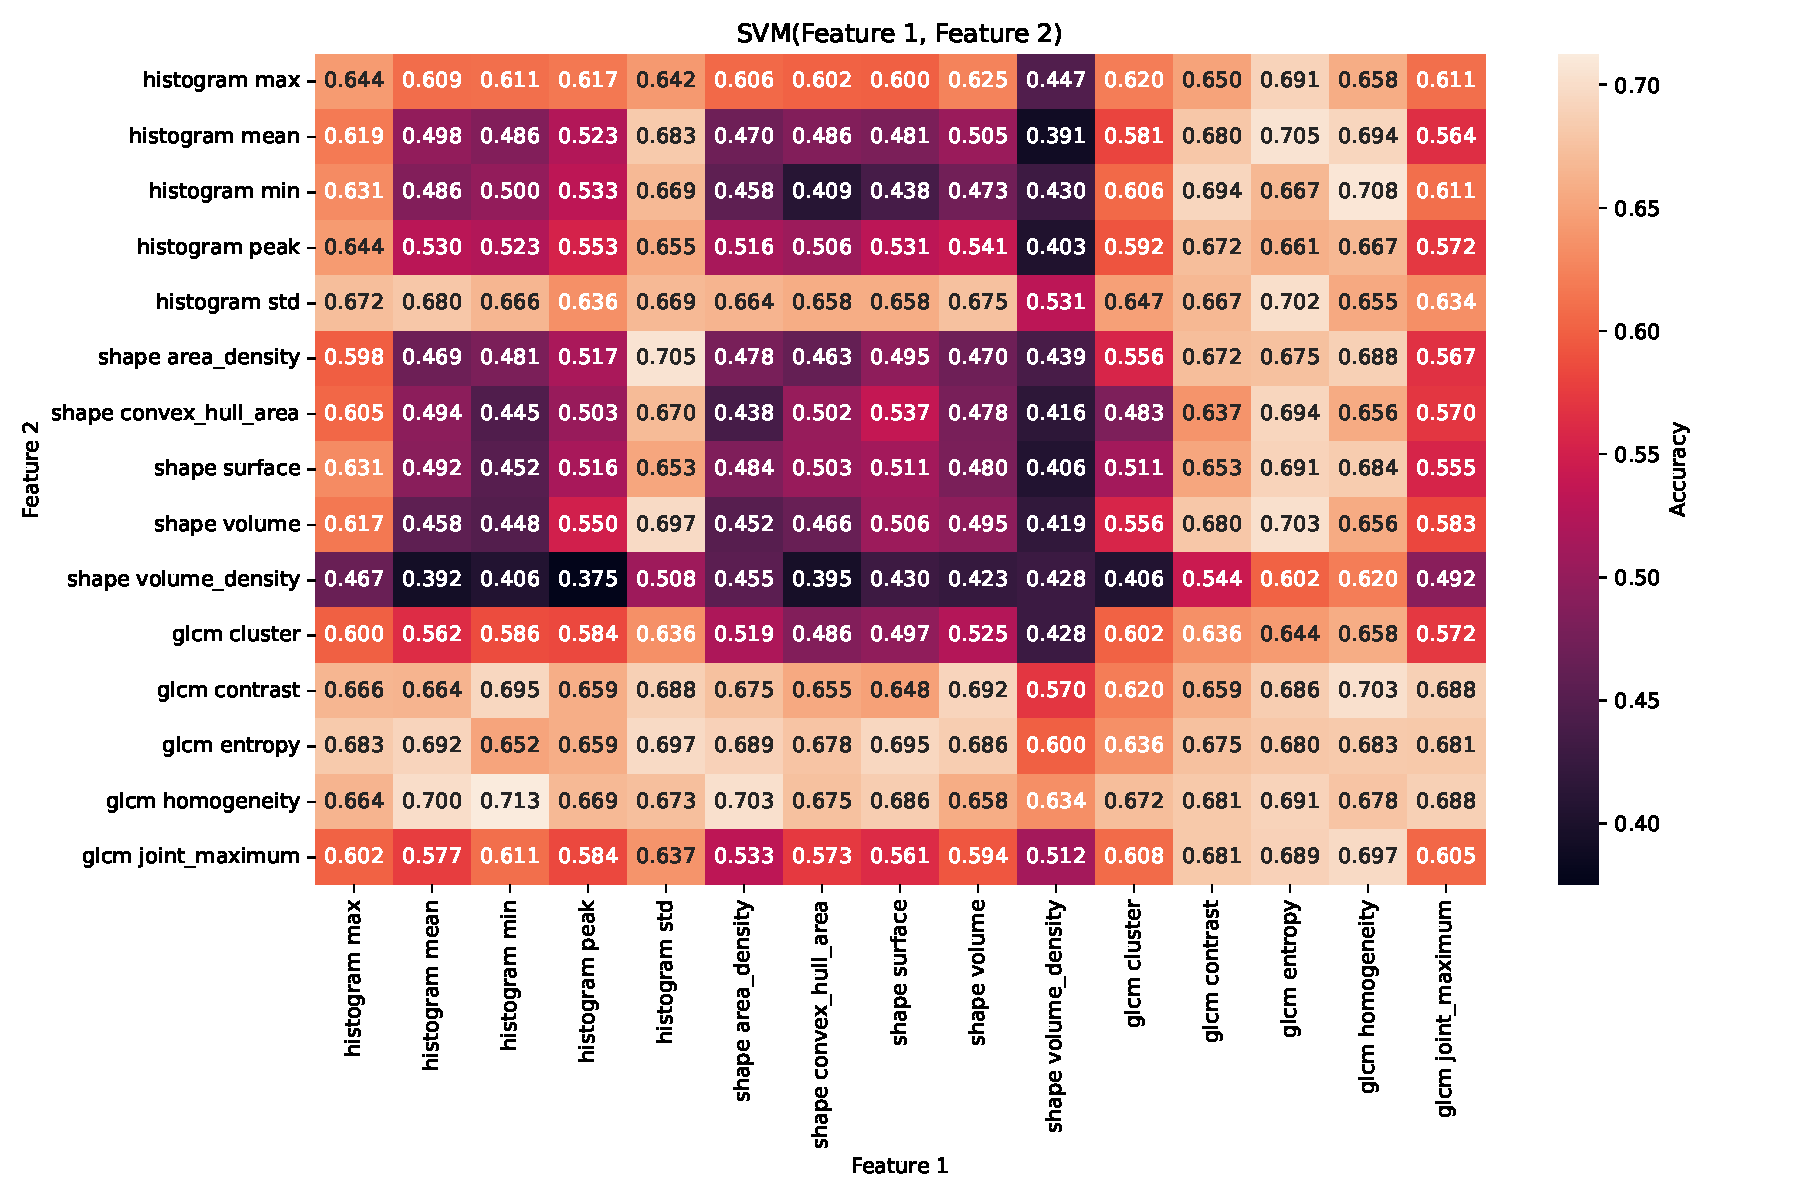
\includegraphics[width=1.2\textwidth]{Figures/feature_pairs4}}
\caption{Heatmap of the accuracy obtained by the SVM model training on different feature pairs. The SVM accuracies are the average 
of $20$ cross-validation cycles training and predicting test data of relative size $0.25$.
The slack constant and GRBF kernel factor are set to $C=10^4$ and $\gamma=1 $ respectively. 
 The predictions are wither the data belongs to series 0 or 1.}
\label{fig:Figures-feature_pairs4}
\end{figure}

\begin{figure}[H]
\centering
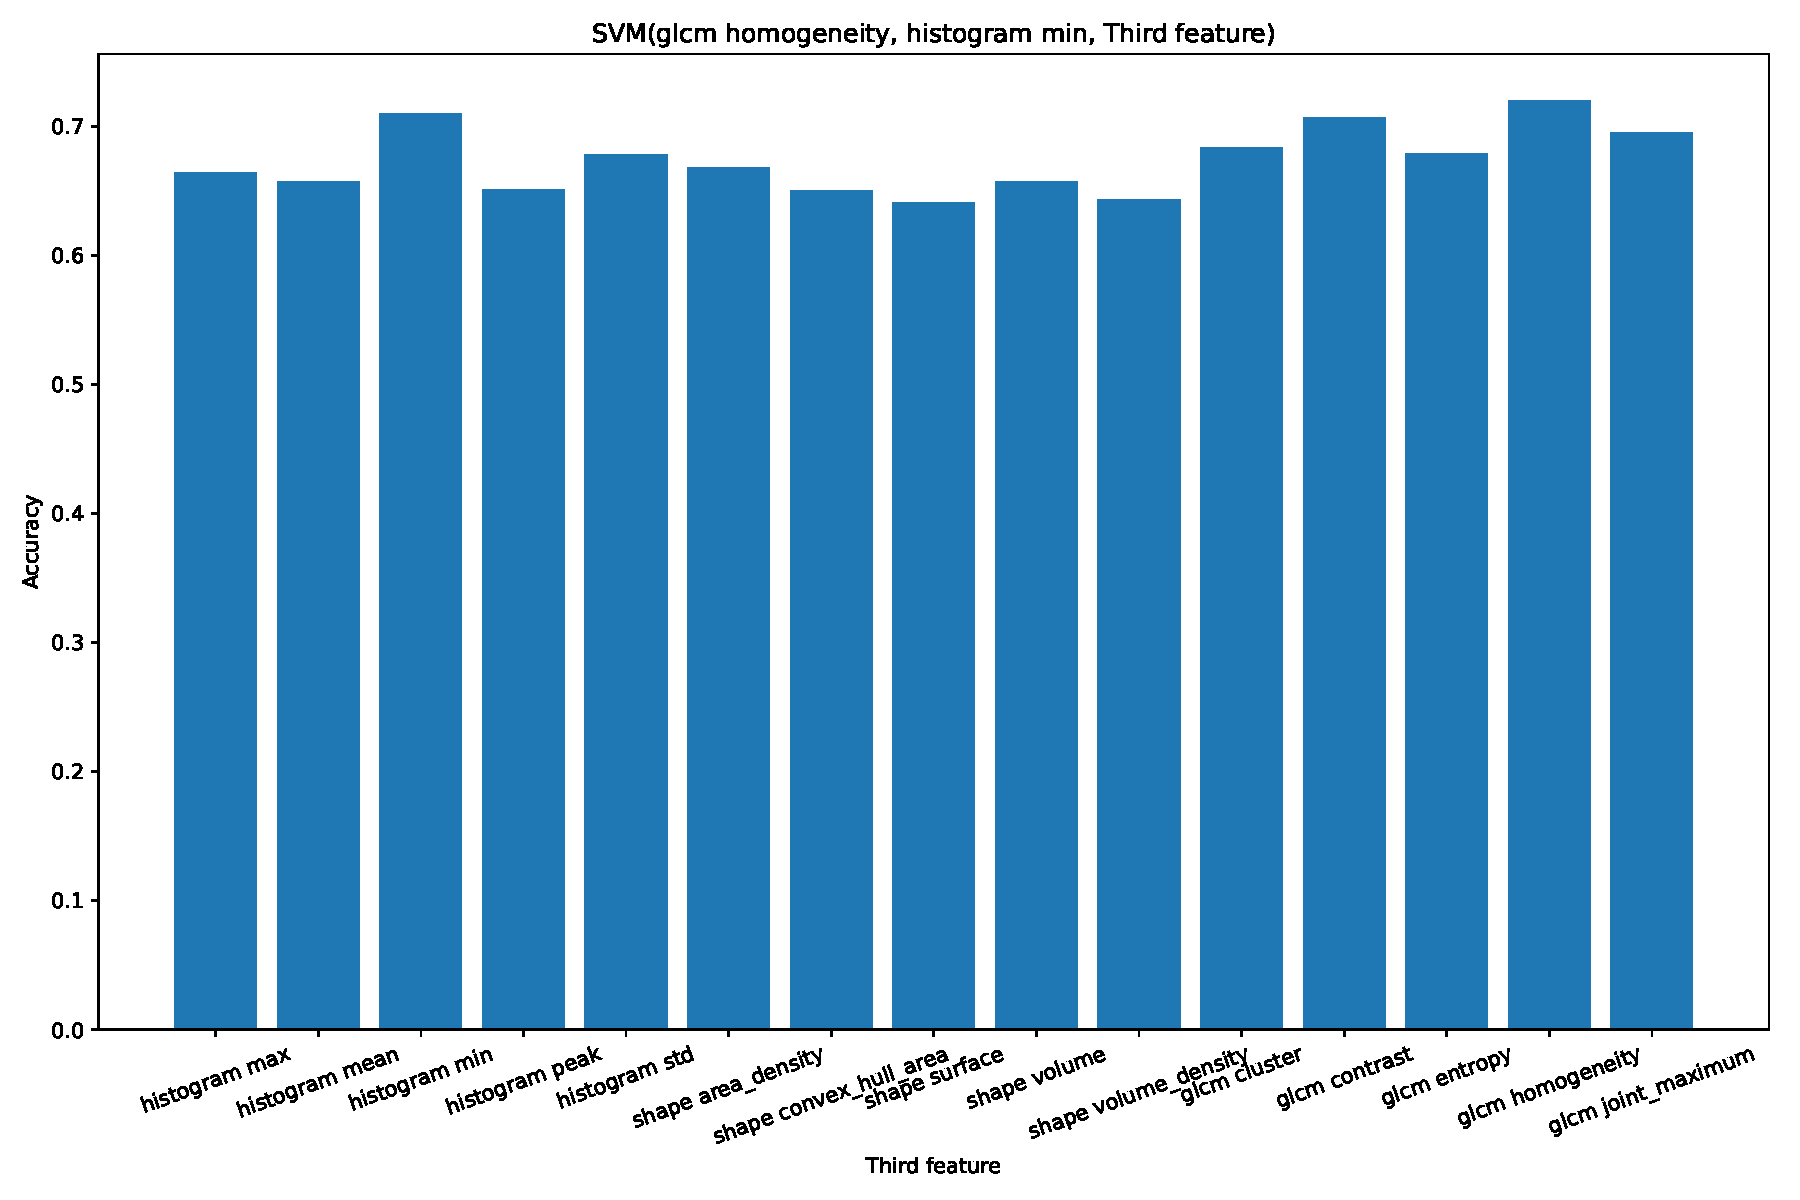
\includegraphics[width=1\textwidth]{Figures/third_feature4}
\caption{Bar plot of the accuracy obtained adding a third feature in the data used 
by the SVM model. The accuracies are the average 
of $50$ cross-validation cycles training and predicting test data of relative size $0.25$.
The slack constant and GRBF kernel factor are set to $C=10^4$ and $\gamma=1 $ respectively.
 The predictions are wither the data belongs to series 0 or 1.}
\label{fig:Figures-third_feature4}
\end{figure}

\autoref{fig:Figures-accuracy-C-gamma-4}-\autoref{fig:Figures-third_feature4} shows the same figures as in \autoref{sec:SVM0} and \autoref{sec:SVM1}, 
but now classifying series 0 versus series 1. From \autoref{fig:Figures-accuracy-C-gamma-4} observe the best accuracy $0.660$ for the 
parameters $C = 10^4$ and $\gamma =1$. Similarly to the analysis classifying series 1 and series 4 in \autoref{sec:SVM0}, the best feature pair is \verb|Histogram min|
and \verb|glcm homogeneity| and the best single feature is \verb|glcm entropy| shown in \autoref{fig:Figures-feature_pairs4}. The addition of a third feature is also similarly 
resulting in worse accuracy as seen from \autoref{fig:Figures-third_feature4}. 

\subsubsection{Series comparison}

The results in \autoref{sec:SVM2} classifying series 0 and 1 are very similar 
to the results in \autoref{sec:SVM0} classifying series 1 and 2 although with worse accuracy. 
The results from \autoref{sec:SVM1} classifying series 0 and 2 are very different, as it shows 
separation for different features. This suggest 
that series 1 is most different and has shifts in some of its features which may be corrected to obtain similar values 
to series 0 and 2. Series 0 and 2 are more similar, but as seen in \autoref{sec:SVM1}, these series 
also have differences in feature values which can be corrected. 


